重力波観測帯域における防振には第\ref{第3章}章で述べたように多段振り子を用いる方法と, 振り子の共振周波数をより低周波にする方法がある. この内, 後者を実現するためにKAGRAでは Inverted Pendulum (IP: 倒立振子)と Geometric Anti-Spring (GAS) フィルタを用いている. これらは反バネ効果(一度変位するとその平衡点から遠ざかろうとするシステム)により振動子の有効バネ定数を低減し, また低い共振周波数を持ちながら, コンパクトな設計となっている. 補遺\ref{補遺A}では主にそれらの動作原理を詳記する. 
\section{IP}
\subsection{動作原理}
IP(倒立振子)は共振周波数を0.1 Hz以下に調整することができる, 水平方向の機械振動子である. これにより, 微小地面振動のピーク周波数(0.2$\sim$0.5 Hz)において1桁程度の減衰を得ることができる. 
\begin{figure}[H]
\begin{center}
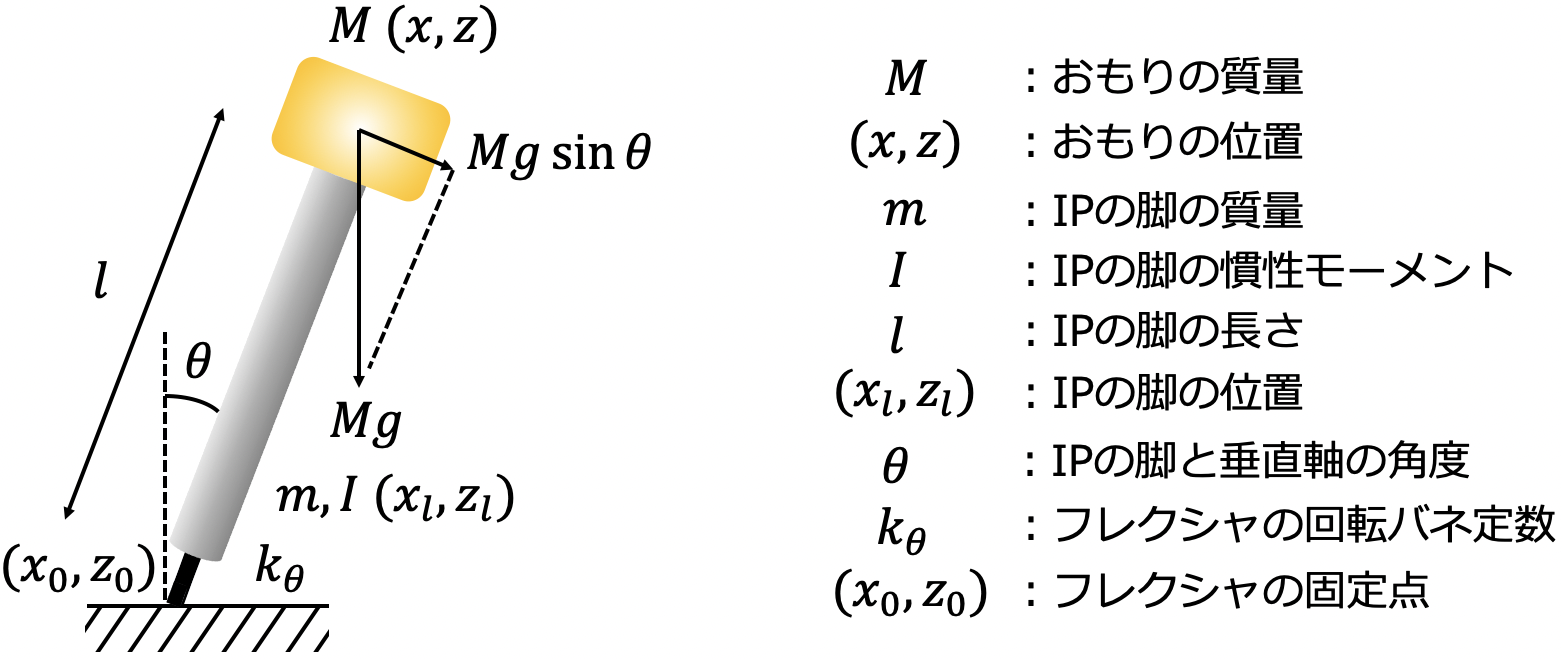
\includegraphics[width=170mm]{figA_1.png} 
\caption[IPの動作原理]{IPの動作原理}
\label{figA.1}
\end{center}
\end{figure}
IPは地面に固定されたフレクシャ, その上に接続された剛性の高い円柱状の脚, および脚の上部にあるおもりから構成される. その簡単なモデルと各パラメータを図\ref{figA.1}に示した. \\
この系のラグランジアン$L$, 運動エネルギー$K$, ポテンシャルエネルギー$U$を計算すると
\begin{equation}
L=K-U,
\end{equation}
\begin{equation}
K=\frac{1}{2}M\left(\dot{x}^2+\dot{z}^2\right)+\frac{1}{2}m\left(\dot{x}_l^2+\dot{z}_l^2\right)+\frac{1}{2}I\ddot{\theta},
\end{equation}
\begin{equation}
U=Mgz+mgz_l+\frac{1}{2}k_{\theta}\theta^2,
\end{equation}
となる. ここで, 
\begin{equation}
\begin{split}
x_l&=\frac{1}{2}(x+x_0)\\
z_l&=\frac{1}{2}z\\
x&=l\sin\theta+x_0\\
z&=l\cos\theta
\end{split},
\end{equation}
という条件を考える. 
\begin{equation}
\begin{split}
\dot{x}&=l\dot{\theta}\cos\theta+\dot{x}_0\\
\dot{z}&=-l\dot{\theta}\sin\theta\\
\end{split},
\end{equation}
であることに注意すると$K$および$U$は
\begin{equation}
K=\frac{1}{2}M\dot{x}^2+\frac{1}{8}m\left(\dot{x}+\dot{x}_0\right)^2+\frac{1}{2}I\left(\frac{\dot{x}-\dot{x}_0}{l}\right)^2,
\end{equation}
\begin{equation}
U=Mgl\cos\left(\frac{x-x_0}{l}\right)+\frac{mgl}{2}\cos\left(\frac{x-x_0}{l}\right)+\frac{1}{2}k_{\theta}\left(\frac{x-x_0}{l}\right)^2.
\label{eqA.7}
\end{equation}
よってEuler-Lagrange方程式は1次近似で
\begin{equation}
\frac{{\rm d}}{{\rm d}t}\frac{\partial K}{\partial\dot{x}}=\frac{\partial U}{\partial x},
\end{equation}
\begin{equation}
\left(M+\frac{m}{4}+\frac{I}{l^2}\right)\ddot{x}+\left(\frac{m}{4}-\frac{I}{l^2}\right)\ddot{x}_0=-\left[\frac{k_{\theta}}{l^2}-\left(M+\frac{m}{2}\right)\frac{g}{l}\right](x-x_0).
\label{eqA.9}
\end{equation}
式(\ref{eqA.9})は有効バネ定数が
\begin{equation}
k_{\rm eff}=\frac{k_{\theta}}{l^2}-\left(M+\frac{m}{2}\right)\frac{g}{l},
\label{eqA.10}
\end{equation}
である調和振動子の運動方程式とみなすことができる. ここで, 式(\ref{eqA.10})の右辺の第1項は弾性復元力を表している.  一方, 第2項は調和振動子の剛性を減少させる斥力(重力反バネ力)を示している. この力はおもりとIPの脚の質量に比例するので, IP上のおもりの質量を変えることで有効バネ定数を調節することができる. \\
\quad しかし, 復元力と斥力を完全に打ち消すと, 系は単一の平衡点を持つ振動系ではなくなってしまう. 各パラメータを表\ref{tableA.1}の通りに仮定すると式(\ref{eqA.7})より, さまざまな荷重をかけたときのIPのポテンシャルエネルギーは図\ref{figA.2}のようになる. 
\begin{table}[H]
 \centering
  \begin{tabular}{cc}
   \hline\hline
   $m$ & 3 kg \\
   $l$ & 2 m \\
   $k_{\theta}$ & 700 N/rad \\
   \hline
  \end{tabular}
 \caption[IPの脚の質量, 長さおよびフレクシャの回転バネ定数]{IPの脚の質量, 長さおよびフレクシャの回転バネ定数. ここではIPの値として適当かつ計算する上で平易な値を定めた. }
 \label{tableA.1}
\end{table}
\begin{figure}[H]
\begin{center}
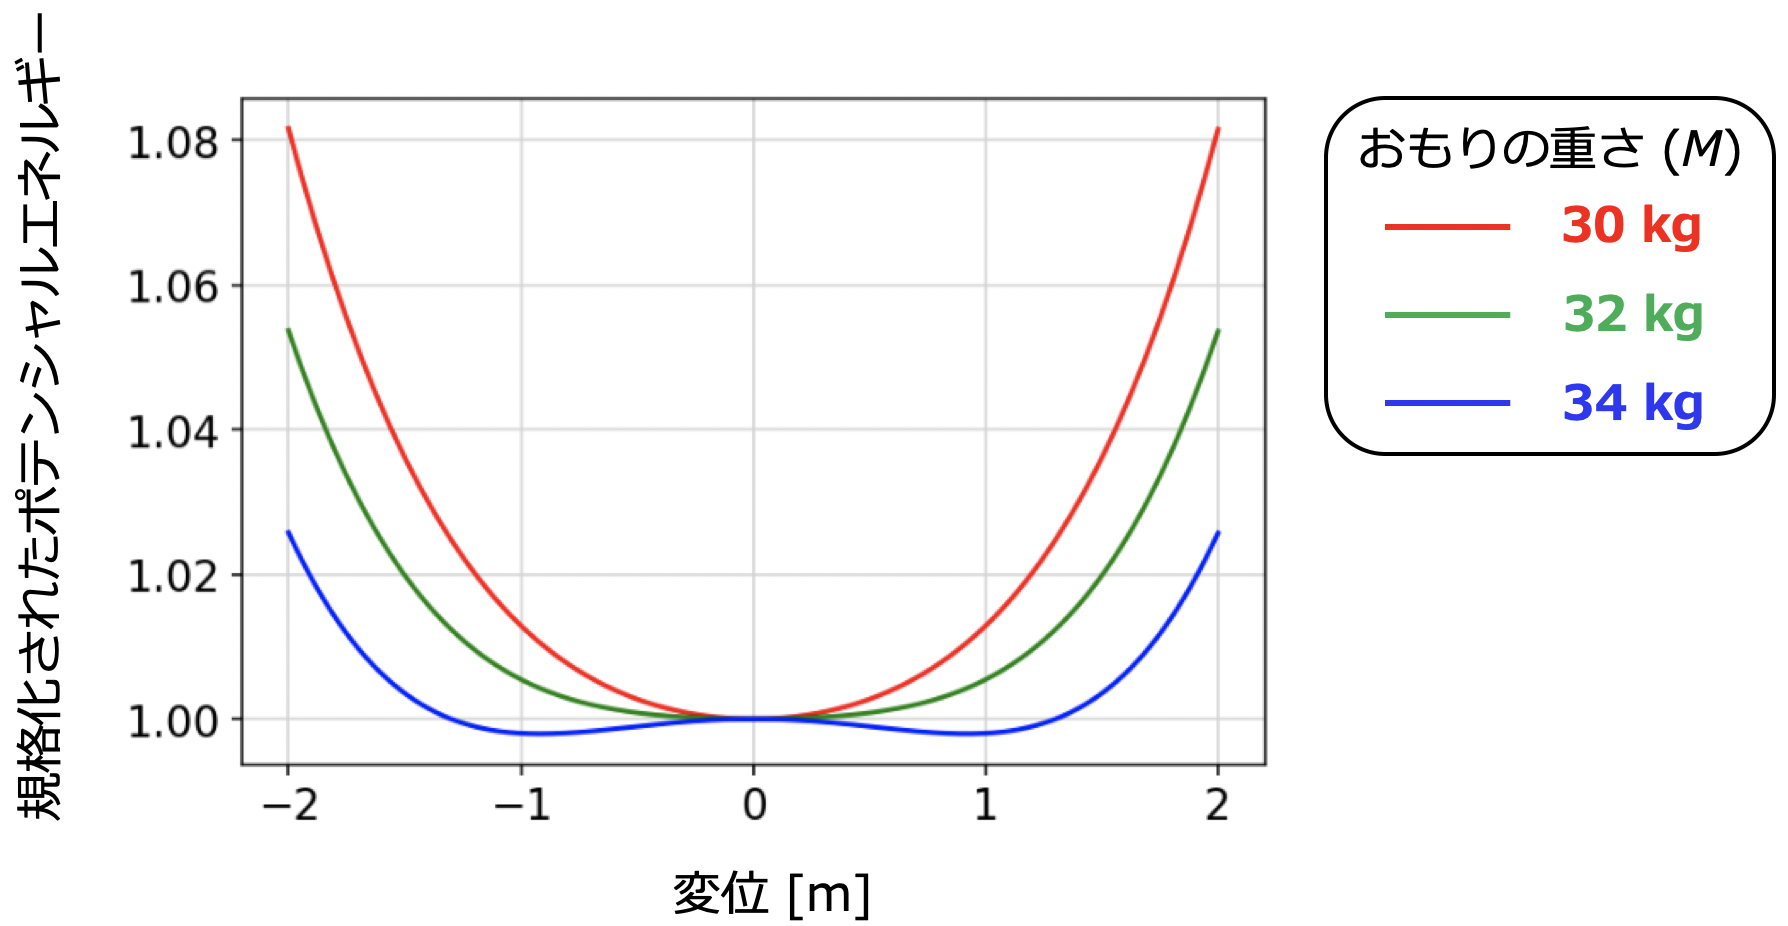
\includegraphics[width=150mm]{figA_2.png} 
\caption[おもりの質量を変えたときのIPのポテンシャルエネルギー]{おもりの質量を変えたときのIPのポテンシャルエネルギー}
\label{figA.2}
\end{center}
\end{figure}
IPに十分な荷重がかかっていない場合, そのポテンシャルエネルギーは式(\ref{eqA.7})の第3項が支配する放物曲線に近似することができる. 荷重が大きくなると, ポテンシャル曲線は平衡点$x=x_0$を中心に平坦になり, 臨界荷重を超えると式(\ref{eqA.7})の第1項が大きくなって, 系は2つの平衡点を持つ双安定性を示すようになる. IPを安定に動作させるためには, 有効バネ定数が正の値になるように荷重を小さくする必要がある. \\
\quad IPが平衡点を1つだけ持つ安定な状態において, IPの共振周波数は式(\ref{eqA.10})より, 
\begin{equation}
f_0=\frac{1}{2\pi}\sqrt{\frac{k_{\rm eff}}{M+\frac{m}{4}+\frac{I}{l^2}}},
\end{equation}
となる. これより, 共振周波数の荷重依存性は図\ref{eqA.3}のようになる. IPにかかる荷重を増加させると共振周波数は徐々に低下し, 最後に急激に低下して系は不安定になることが分かる. 
\begin{figure}[H]
\begin{center}
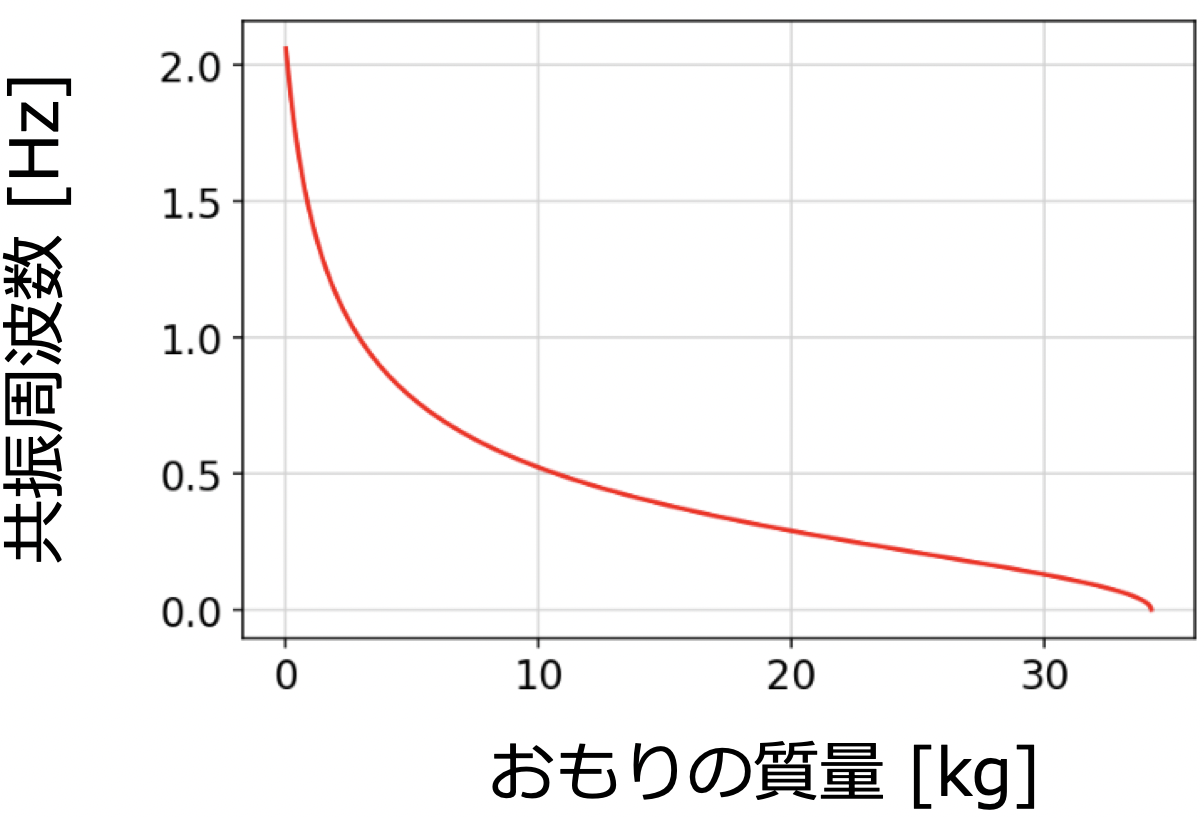
\includegraphics[width=120mm]{figA_3.png} 
\caption[おもりの質量を変えたときのIPの共振周波数の変化]{おもりの質量を変えたときのIPの共振周波数の変化}
\label{figA.3}
\end{center}
\end{figure}
\subsection{減衰性能}
IPの脚が均一な質量分布だと仮定すると, 地面からおもりへの伝達関数は
\begin{equation}
H_{\rm IP}(\omega)=\frac{\tilde{x}}{\tilde{x}_0}.
\label{eqA.12}
\end{equation}
ここで, Euler-Lagrange方程式(\ref{eqA.9})より
\begin{equation}
\left[k_{\rm eff}-\left(M+\frac{m}{4}+\frac{I}{l^2}\right)\omega^2\right]\tilde{x}=\left[k_{\rm eff}-\left(\frac{m}{4}-\frac{I}{l^2}\right)\omega^2\right]\tilde{x}_0,
\label{eqA.13}
\end{equation}
なので
\begin{equation}
H_{\rm IP}(\omega)=\frac{k_{\rm eff}-\left(\frac{m}{4}-\frac{I}{l^2}\right)\omega^2}{k_{\rm eff}-\left(M+\frac{m}{4}+\frac{I}{l^2}\right)\omega^2}=\frac{A+B\omega^2}{A-\omega^2}.
\end{equation}
ただし, 
\begin{equation}
A=\frac{k_{\rm eff}}{M+\frac{m}{4}+\frac{I}{l^2}},\quad B=\frac{\frac{m}{4}-\frac{I}{l^2}}{M+\frac{m}{4}+\frac{I}{l^2}},
\end{equation}
である. ここで, $H_{\rm IP}(\omega)$の振幅を周波数の関数として描くと図\ref{figA.4}のようになる. ある周波数までは理想的なバネと同様であるが, 高周波数で減衰性能が飽和するのが分かる. これは式(\ref{eqA.12})に示した係数Bによるものである. 
\begin{figure}[H]
\begin{center}
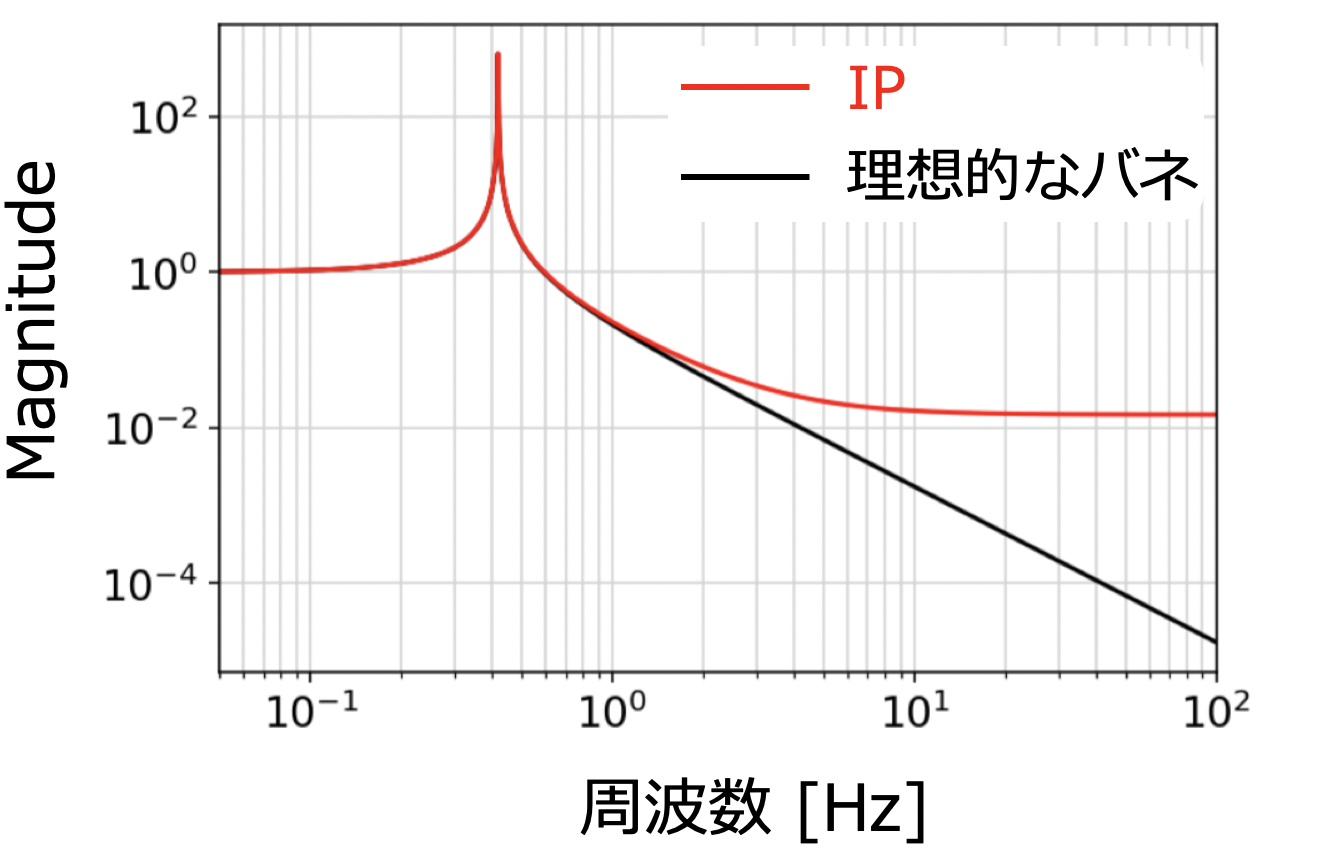
\includegraphics[width=140mm]{figA_4.png} 
\caption[地面の運動からIPのおもりまでの伝達関数]{地面の運動からIPのおもりまでの伝達関数. 黒線は理想的なバネの場合である. }
\label{figA.4}
\end{center}
\end{figure}
係数Bによる飽和状態は, 物理的には打撃中心効果\cite{cop}による脚部からおもりへの運動量伝達である. 剛体に衝撃的な力を加えると, 図\ref{figA.5}に示すように, 打撃によって剛体はその重心の移動と重心周りの回転の両方で加速される. このとき, 並進と回転が相殺され, 正味の初速度がゼロになる点が存在する. この点をピボットポイント, あるいはスイートスポットと呼び, 衝動の瞬間的な回転中心と見なすことができる. なお, ピボットポイントの位置は物体の質量分布によって決まる. \\
\quad ピボットポイントは重心の反対側に打撃中心点(CoP, Center of Percussion)を持つ. ここで, CoPに垂直な打撃を加えても, それに対応するピボットポイントには反作用の力が発生しない. CoPとピボットポイントの質量中心からの距離$r_{\rm f}$と$r_{\rm p}$は
\begin{equation}
r_{\rm f}r_{\rm p}=\frac{I_{\rm body}}{M_{\rm body}},
\label{figA.5}
\end{equation}
で表される\cite{cop}. ここで, $M_{\rm body}$と$I_{\rm body}$はそれぞれ物体の質量と慣性モーメントである. この関係から重心の反対側に衝撃が加わると, CoPとピボットポイントの位置が入れ替わることが分かる. \\
\quad IPの脚の場合, 一端がおもりに接続され, もう一端がフレクシャを介して地面に固定されているため, 自由に回転できないという機械的制約がある. これにより, IPは低周波で共振する調和振動子のような振る舞いをする. しかし, 周波数が高くなるとこの制約は弱くなり, IPの脚はピボットポイントを中心に自由に回転することができるようになる. 脚からおもりへの運動量伝達を低減するためには, IPの脚の上端に相当するCoPの位置を, 外力(地面の運動)が加わるフレクシャの足と一致させる必要がある. これによりIPの脚はおもりに力を与えることなく, その上端を支点として回転することができる. \\
\quad 前述の通り, CoPの位置(ピボットポイントの位置)は剛体の質量分布に依存するため, IPの脚の下部にカウンターウェイトを追加することでCoPの位置を調整している(図\ref{figA.6}). カウンターウェイトはおよそ1$\sim$2桁の飽和レベルの緩和が可能であり, 例えばAdvanced LIGO用に開発されたHAM-SASのIPはカウンターウェイトなしで$\sim10^{-3}$の減衰, カウンターウェイトありでは$\sim10^{-5}\sim10^{-4}$の減衰を達成した. 図\ref{figA.7}にカウンターウェイトの導入による防振比の飽和レベルの改善を示す. 
\begin{figure}[H]
\begin{center}
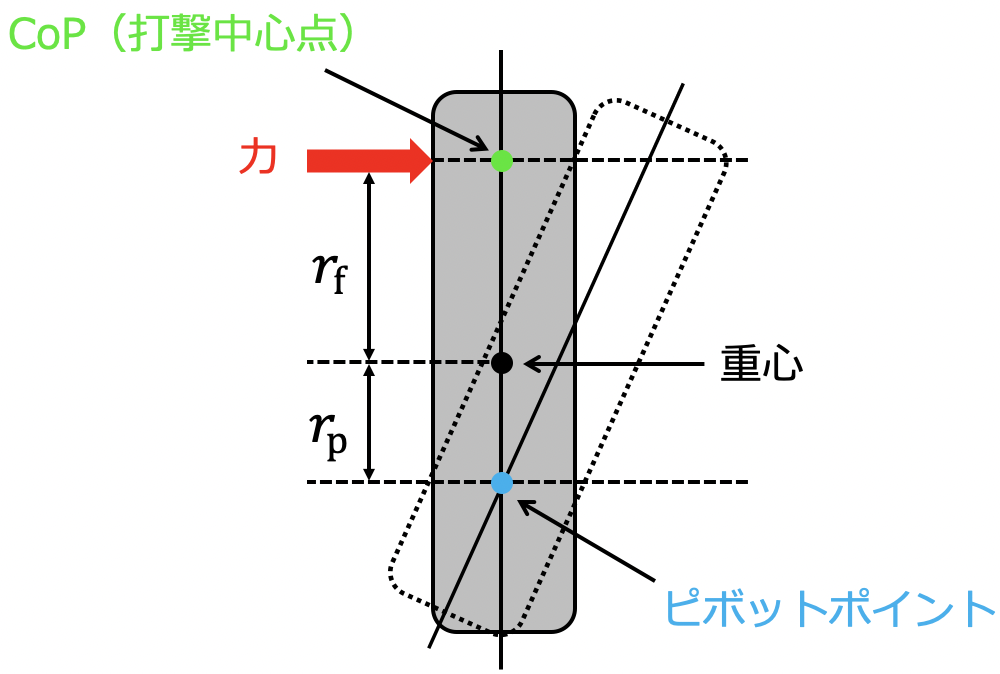
\includegraphics[width=130mm]{figA_5.png} 
\caption[CoP (Center of Percussion)]{CoP (Center of Percussion)の図. 剛体は重心から外れた箇所に衝撃力を受けると, 重心の並進と重心周りの回転の両方で瞬間的な加速度を持つ. このとき, 並進と回転が打ち消しあって正味の初速がゼロになる点(ピボットポイント)が存在する. CoPは重心に対してピボットポイントの反対側に位置する補点である. つまりCoPとは, 与えられたピボットポイントにおいて垂直方向の衝撃による反力が発生しないような点である. }
\label{figA.5}
\end{center}
\end{figure}
\begin{figure}[H]
\begin{center}
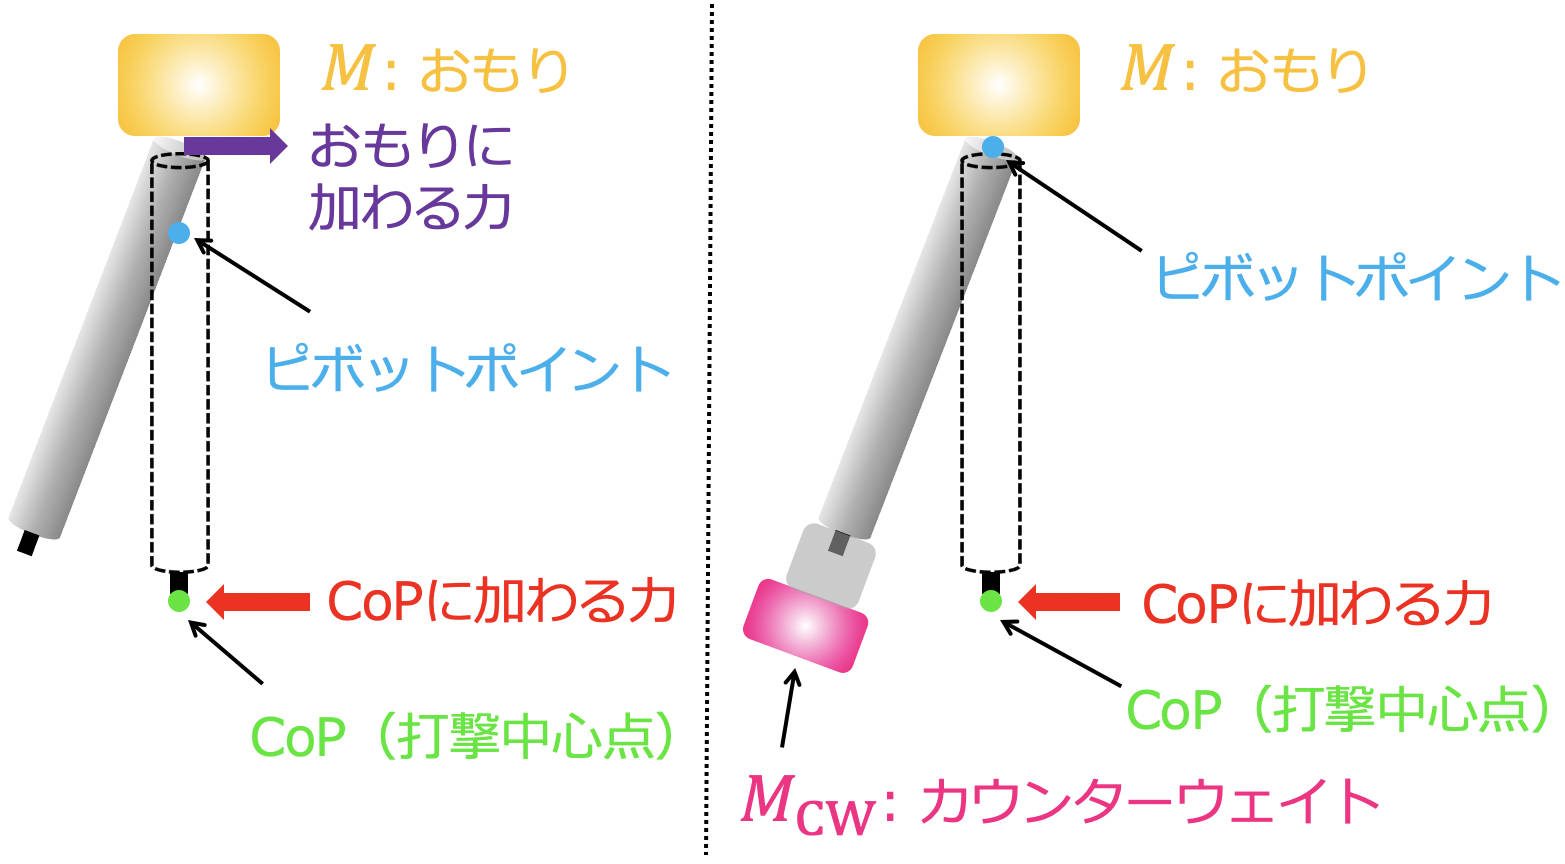
\includegraphics[width=150mm]{figA_6.png} 
\caption[カウンターウェイト]{カウンターウェイトを設置したものとそうでないものの比較図. 一般に, 下部のフレクシャ部分に位置するCoPと相補的なピボットポイントは, ペイロードの連結部とは一致しない. このため, カウンターウェイトを脚の下部に設置することで, ピボットポイントを上部の連結部と一致させ, おもりに力をかけずにIPの脚を回転させ, 地面からの分離性能を向上させている. }
\label{figA.6}
\end{center}
\end{figure}
\begin{figure}[H]
\begin{center}
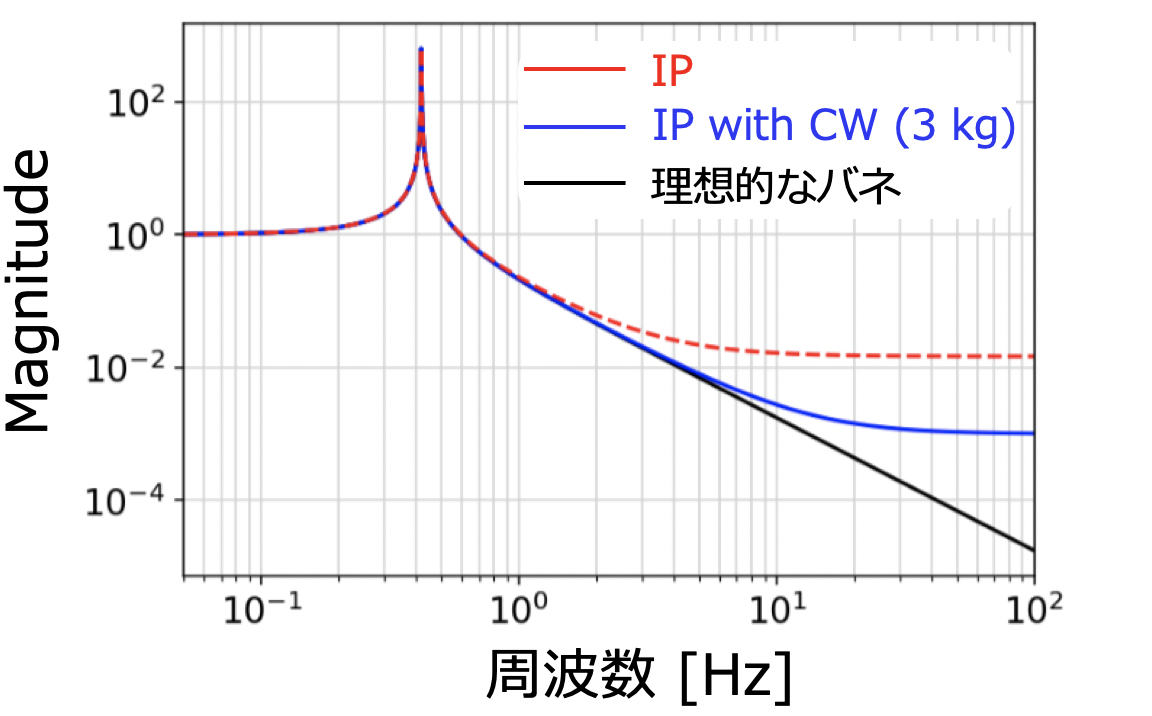
\includegraphics[width=150mm]{figA_7.png} 
\caption[カウンターウェイトの質量を変えたときのIPの防振比]{カウンターウェイトの質量を変えたときのIPの防振比. カウンターウェイトにより, 飽和レベルが1$\sim$2桁向上していることが分かる. }
\label{figA.7}
\end{center}
\end{figure}
\section{GASフィルタ}
低周波において, 垂直方向の防振を実現するためには柔らかいバネを用いる必要があるが, そのバネは懸架系の重量を支えられるものでなくてはならない. そこでVirgoではSuper Attenuatorに磁気反バネ技術を導入していた. これは同じ磁極を持つ永久磁石を水平面内で向かい合わせ, その反発力を用いるものである. 磁石が垂直方向に変位した時に反発力が垂直方向に伝わり, それがバネの反発力となって垂直バネの剛性を低下させる. しかし, 磁場の強さは温度に強く依存するため, 温度変化に伴って共振周波数がずれてしまう. さらに, 永久磁石やセンタリングに使う装置の影響で余計な機械的共振が誘発され, 観測帯域における防振性能が低下するという問題もあった. \\
\quad この磁気バネを改良したものがGAS (Geometric Anti-Spring) フィルタである\footnote{Geometric Anti-Spring の名称は, 反バネが板バネの特定の形状によって実現されていることを表している. }
. これは2等辺三角形の板ばねを頂点で結合し, 3方向から均等に圧縮する機械振動子であり, 低周波の垂直共振を約0.3 Hzで抑えることができる. これにより防振性能が向上しただけでなく, 熱安定性やより簡素な機構が得られた. 以下ではその動作原理や機械的特性について述べる. 
\subsection{動作原理}
GASフィルタの構造は\ref{sec4.1.1.2}で示した通りであり, 準三角形の板バネがその頂点で互いに圧縮しながら接続されている. この圧縮により垂直変位に対して反発力が生まれるのである. \\
\quad ここで, 垂直バネと水平バネの組み合せで懸架系を支えて互いに圧縮するシステムとしてGASフィルタをモデル化する(図\ref{figA.8}). ここで, 板バネが放射状に, かつ対称に設置されているため, 圧縮に対する反力の水平成分は消失し, キーストーンは垂直方向のみに動くよう拘束されている. 
\begin{figure}[H]
\begin{center}
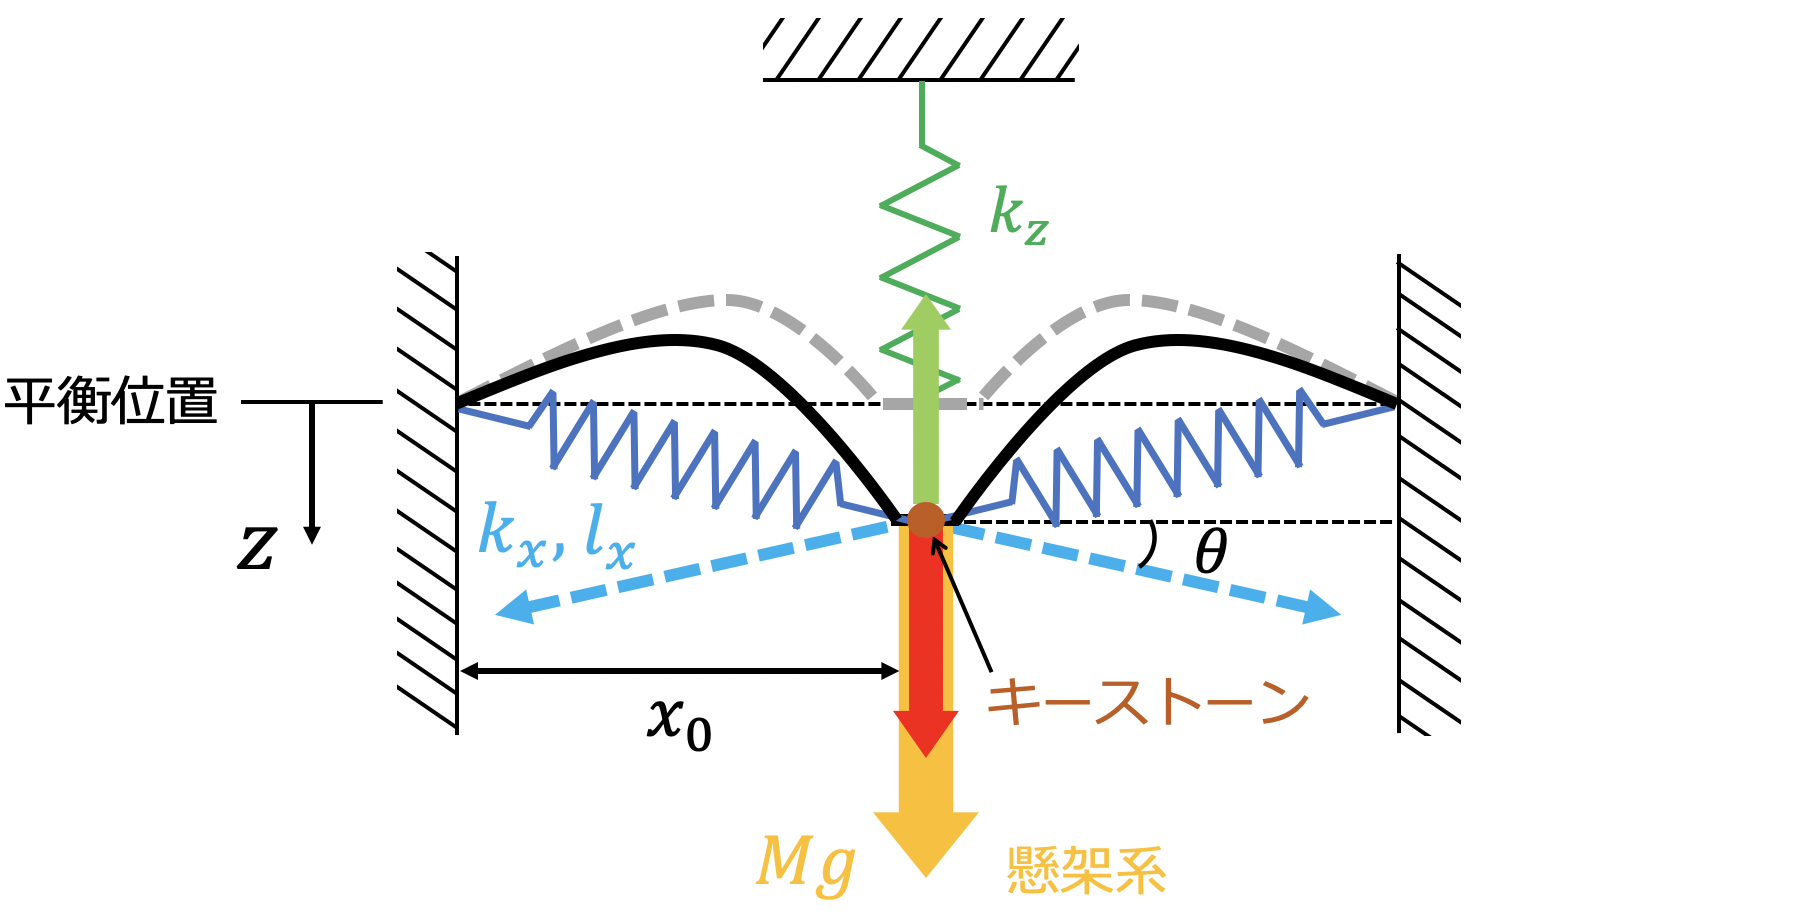
\includegraphics[width=160mm]{figA_8.png} 
\caption[GASフィルタの概略図]{GASフィルタの概略図. 1組の板バネが互いに圧縮され, キーストーン(茶)を支えている. この系は通常の垂直バネ(緑)と圧縮された水平バネ(青)の組み合わせでモデル化することができる. キーストーンが変位すると, 圧縮に対する反力の水平成分は互いに打ち消し合い(水色の点線矢印), $z$軸に沿った正味の反発力(赤の矢印)が残る. 結果としてキーストーンの剛性は, 垂直バネと正味の水平バネの寄与の合計となる. }
\label{figA.8}
\end{center}
\end{figure}
GASフィルタのキーストーンが平衡位置$z=z_{\rm eq}$にあるとき$Mg$ ($M$:懸架系の質量)とバネの力が釣り合っており, 水平バネは$z$軸に直交 ($\theta=0$) して, 最も圧縮される. キーストーンが平衡状態から変位すると運動方程式は
\begin{equation}
M\ddot{z}=-k_z(z-z_{\rm eq})-k_x(l_x-l_{x0})\sin\theta.
\label{eqA.17}
\end{equation}
ここで$k_z, k_l$はそれぞれ垂直, 水平バネのバネ定数であり, $l_x, l_{x_0}$は水平バネの位置およびその元の位置である. $z_{\rm eq}$の周りで式(\ref{eqA.17})を$z$の1次で展開すると, 以下のように線形化できる. 
\begin{equation}
M\ddot{z}=\left[k_z-\left(\frac{l_{x0}}{x_0}-1\right)k_x\right](z-z_{\rm eq})=-k_{\rm eff}(z-z_{\rm eq}).
\end{equation}
ここで, $x_0$はキーストーンと水平バネの支点の水平距離であり, また有効バネ定数は
\begin{equation}
k_{\rm eff}=k_z-\left(\frac{l_{x0}}{x_0}-1\right)k_x,
\end{equation}
とした. 水平ばねが圧縮されているとき ($x_0<l_{x0}$), 垂直方向に反発力が発生するため有効バネ定数は垂直バネのバネ定数($k_{\rm eff}<k_z$)より小さくなる. これが, GASスプリングのアンチスプリング効果の原理であり, ブレードの圧縮を大きくする($x_0$を小さくする)ことで実効剛性と共振周波数を小さくすることができる. 
\subsection{減衰性能}
基準フレームの垂直変位からキーストーンへのGASフィルタの伝達関数は, IPの場合と同じ式(\ref{eqA.13})で表される. GASフィルタの場合もCoP効果によって減衰性能は高周波数で飽和し, 一般に$\sim10^3$が限界となる\cite{attenuate}. しかし, マジックワンド(図\ref{fig4.3})を追加することで減衰レベルを$10^4$まで向上させることができる. 
\subsection{熱ドリフト}
GASフィルタは水平圧縮力と板バネの固有垂直剛性による反バネ効果のバランスを取ることで, 大きな柔性を得ている. この柔性により, 懸架系の質量やバネの物性のわずかな変化に対して, キーストンの垂直位置が変動する. 特に, バネの材質のヤング率の温度依存性による熱ドリフトは, GASフィルタを運用する上で大きな問題となる. \\
\quad GASフィルタの動作点に懸架系の質量$M$で釣り合った場合, その位置にキーストーンを保つための最適荷重は, 温度変化により次のようにずれる. 
\begin{equation}
\Delta M\approx\frac{M}{E}\frac{\partial E}{\partial T}\Delta T.
\end{equation}
ここで, $E$はバネの材質のヤング率であり, $\Delta T$は温度変化である. 小さな摂動の場合, この変化はキーストーンに追加される力$\Delta F=\Delta Mg$と等価である. この系は有効バネ定数$k_{\rm eff}$を持つので, 熱変化による変位は
\begin{equation}
\Delta z=\frac{\Delta F}{k_{\rm eff}}=\frac{g}{E\omega_0^2}\frac{\partial E}{\partial T}\Delta T.
\end{equation}
ここで, GASフィルタの共振周波数は$\omega_0$に調整されているため, 有効バネ定数は$k_{\rm eff}=M\omega_0^2$として計算される. 反バネ効果により共振周波数が低下すると, 系は温度変化に対してより敏感になる. 典型的なパラメータを用いた場合, 温度依存性は
\begin{equation}
\frac{\Delta z}{\Delta T}=0.69\,\,[\rm{mm/K}]\left(\frac{0.33 \rm{Hz}}{\omega_0/2\pi}\right)^2\left(\frac{\frac{1}{E}\frac{\partial E}{\partial T}}{3.0\times10^{-4}[\rm{1/K}]}\right),
\end{equation}
となる. 




